\documentclass[fleqn, 11pt]{beamer}
\usepackage{amsmath}
\usepackage{amssymb}
\usepackage{geometry}
\usepackage{graphicx}
\usepackage{url}
\usepackage{xcolor}
\usepackage{enumerate}

% some latex magic for correcting apostrophe issue in verbatim mode
\makeatletter
\let \@sverbatim \@verbatim
\def \@verbatim {\@sverbatim \verbatimplus}
{\catcode`'=13 \gdef \verbatimplus{\catcode`'=13 \chardef '=13 }} 
\makeatother

\begin{document}

%---------------------------------------------
\begin{frame}
\large
Lecture 8:\\
Hypothesis Testing for a Proportion\\
STAT 310, Spring 2021
\normalsize
\end{frame}

%---------------------------------------------
\begin{frame}{Hypothesis Test for a Proportion}
\textbf{Key components:}
\vspace{5pt}
\begin{itemize}
\item Null hypothesis:\\
$H_0: p = p_0$
\vspace{5pt}
\item Alternative hypothesis (use one of these):\\
$H_A: p > p_0$ (one-sided, upper-tail)\\
$H_A: p < p_0$ (one-sided, lower-tail)\\
$H_A: p \neq p_0$ (two-sided)
\vspace{5pt}
\item Test statistic:
\begin{align*}
z = \frac{\text{observed value} - \text{null value}}{\text{SE}} = 
\frac{\hat{p} - p_0}{\sqrt{\frac{p_0(1-p_0)}{n}}}
\end{align*}
\item A rule to either reject or not reject $H_0$
\end{itemize}
\end{frame}

%---------------------------------------------
\begin{frame}{Hypothesis Testing Concept}
The approach to hypothesis testing is as follows:
\vspace{5pt}
\begin{enumerate}
\item Assume that $H_0$ is true.  $H_0$ usually represents a skeptical position, or a perspective of no difference or change in the parameter of interest.
% corresponds to no real effect
\vspace{5pt}
\item Reject $H_0$ only if the data provide strong evidence in support of the alternative claim in $H_A$.\\
\end{enumerate}
\end{frame}

%---------------------------------------------
\begin{frame}{Hypothesis Testing Concept}
The hypothesis testing framework can be found in the US court system, where innocence is assumed until proven guilty.\footnote{\tiny \url{https://commons.wikimedia.org/wiki/File:Trial_of_Edward_Ellis_(courtroom_sketch).jpg}}\\
\vspace{5pt}
$H_0$:  The defendant is innocent.\\
$H_A$:  The defendant is guilty.\\
\vspace{5pt}
The jurors consider whether the evidence is convincing enough to convict the defendant (reject $H_0$).\\
\flushright
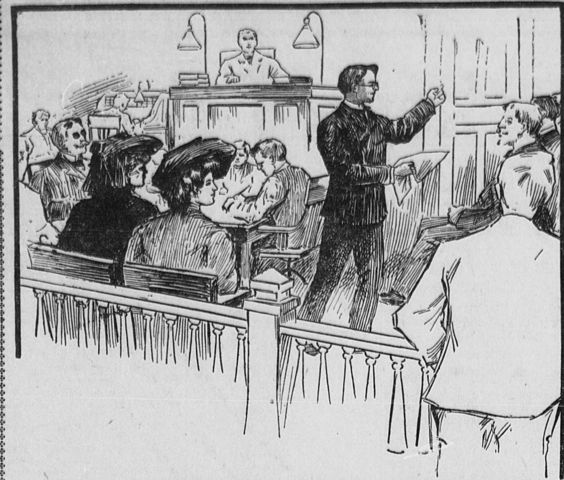
\includegraphics[scale=0.2]{figure/courtroom_sketch.jpg}
\end{frame}

%---------------------------------------------
\begin{frame}{$p$-value}
A \textbf{$p$-value} is the probability of obtaining a test statistic as extreme, or more extreme (in the direction of the alternative), than the observed value of the test statistic, assuming that $H_0$ is true.\\
\end{frame}

%---------------------------------------------
\begin{frame}{$p$-value}
Decision rule using the $p$-value:
\vspace{5pt}
\begin{itemize}
\item If $p$-value $< \alpha$, then reject $H_0$.
\item If $p$-value $> \alpha$, then do not reject $H_0$.
\end{itemize}
\vspace{10pt}
$\alpha$ is called the \textbf{signficance level}.  Common values for $\alpha=0.05, 0.01$\\
\end{frame}

%---------------------------------------------
\begin{frame}{$p$-value}
\begin{itemize}
\item When the $p$-value $< \alpha$ (we reject $H_0$) the result is said to be \textbf{statistically significant}.
\vspace{10pt}
\item In other words, a result is statistically significant when it is unlikely to of occurred by random chance, assuming that the null hypothesis is true.
\vspace{10pt}
\item The smaller the $p$-value, the stronger the data favor $H_A$ over $H_0$.
\end{itemize}
\end{frame}

%---------------------------------------------
\begin{frame}{Computing $p$-values}
\begin{columns}
\begin{column}{0.45\textwidth}
%\large
One-sided test (upper-tail):\\
$H_0: p = p_0$\\
$H_A: p > p_0$\\
\vspace{10pt}
Test statistic:\\
\[ z = \frac{\hat{p} - p_0}{\sqrt{\frac{p_0(1-p_0)}{n}}} \]\\
\vspace{10pt}
$p$-value $= \texttt{1 - pnorm(z)}$\\ 
\vspace{10pt}
Reject $H_0$ if $p$-value $< \alpha$\\
\end{column}
\begin{column}{0.5\textwidth}
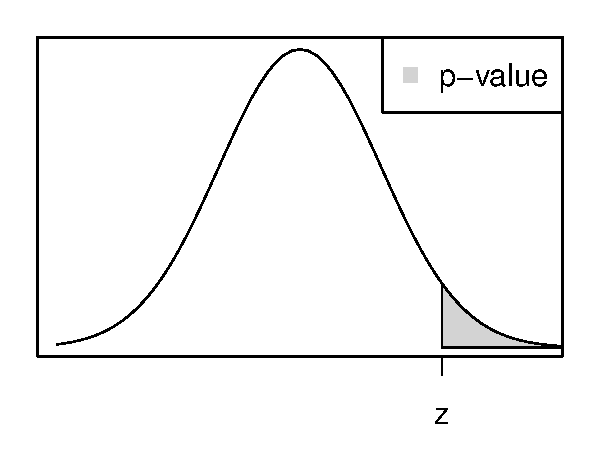
\includegraphics[scale=0.5]{figure/pvalue_upper.pdf}
\end{column}
\end{columns}
\end{frame}

%---------------------------------------------
\begin{frame}{Computing $p$-values}
\begin{columns}
\begin{column}{0.45\textwidth}
%\large
One-sided test (lower-tail):\\
$H_0: p = p_0$\\
$H_A: p < p_0$\\
\vspace{10pt}
Test statistic:\\
\[ z = \frac{\hat{p} - p_0}{\sqrt{\frac{p_0(1-p_0)}{n}}} \]\\
\vspace{10pt}
$p$-value $= \texttt{pnorm(z)}$\\ 
\vspace{10pt}
Reject $H_0$ if $p$-value $< \alpha$\\
\end{column}
\begin{column}{0.5\textwidth}
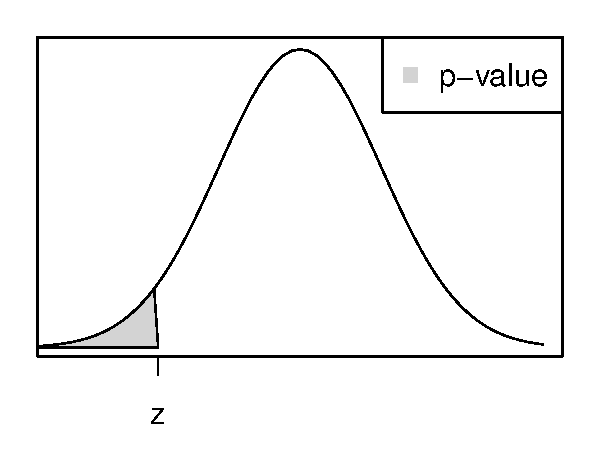
\includegraphics[scale=0.5]{figure/pvalue_lower.pdf}
\end{column}
\end{columns}
\end{frame}

%---------------------------------------------
\begin{frame}{Computing $p$-values}
\begin{columns}
\begin{column}{0.55\textwidth}
%\large
Two-sided test:\\
$H_0: p = p_0$\\
$H_A: p \neq p_0$\\
\vspace{10pt}
Test statistic:\\
\[ z = \frac{\hat{p} - p_0}{\sqrt{\frac{p_0(1-p_0)}{n}}} \]\\
\vspace{10pt}
$p$-value $= \texttt{2*pnorm(-abs(z))}$\\ 
\vspace{10pt}
Reject $H_0$ if $p$-value $< \alpha$\\
\end{column}
\begin{column}{0.45\textwidth}
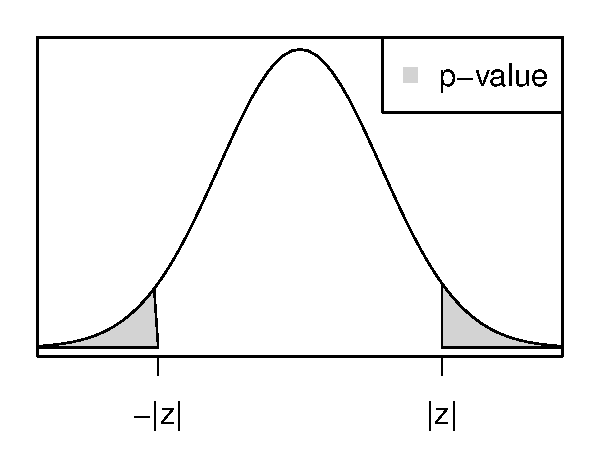
\includegraphics[scale=0.5]{figure/pvalue_both.pdf}
\end{column}
\end{columns}
\end{frame}

\begin{frame}{Conditions}
A hypothesis test for a proportion is valid if the following conditions are satisfied:\\
\begin{itemize}
\item The data were collected using simple random sampling
\item $n p_0 \geq 10$ and $n(1-p_0) \geq 10$
\end{itemize}

\vspace{10pt}
These conditions ensure that the Central Limit Theorem holds.  So, assuming that $H_0$ is true, the sampling distribution for $\hat{p}$ is approximately normal with mean $p_0$ and standard error $\sqrt{p_0 (1-p_0) / n}$.
\end{frame}

\begin{frame}{Example} % One-sided
\small
A simple random sample of 1,028 US adults in March 2013 found that 56\% support nuclear arms reduction. Does this provide convincing evidence that a majority of Americans support nuclear arms reduction?
\begin{enumerate}[(a)]
\item Write the null and alternative hypothesis for a one-sided test.\\
\vspace{1.5cm}
\item Check the conditions for the hypothesis test.
\vspace{1.5cm}
\item Calculate the test statistic.\\
\vspace{2cm}
\end{enumerate}
\end{frame}

\begin{frame}{Example} % One-sided
\small
A simple random sample of 1,028 US adults in March 2013 found that 56\% support nuclear arms reduction. Does this provide convincing evidence that a majority of Americans support nuclear arms reduction?
\begin{enumerate}[(a)]
\setcounter{enumi}{3}
\item Calculate the $p$-value and make a decision using $\alpha = 0.05$\\ significance level.
\vspace{2.25cm}
\item What is the conclusion of the test in the context of the data?\\
\vspace{2.25cm}
\end{enumerate}
\end{frame}

% \begin{frame}{Example 2} % Two-sided
% 400 students were randomly sampled from a large univeristy, and 289 said they did not get enough sleep.  Conduct a hypothesis test to check whether this represents a statistically significant difference from 50\%, and use a significance level of 0.01.
% \end{frame}

%---------------------------------------------
\begin{frame}{Decision Errors}
\begin{table}[ht]
\begin{tabular}{p{3cm}|p{3cm}|p{3cm}}
 & Do not reject $H_0$ &  Reject $H_0$\\
\hline
$H_0$ true \newline &  & \\
\hline
$H_A$ true \newline  &  &\\ 
\end{tabular}
\end{table}

\vspace{20pt}
The significance level of the test, $\alpha$, is the probability of a type I error (probability of rejecting $H_0$ when $H_0$ is true).
\end{frame}

%---------------------------------------------
\begin{frame}{Decision Errors}
\vspace{-3cm}
In a US court, the defendant is either innocent ($H_0$) or guilty ($H_A$).  What does a type I error represent in this context?  What does a type II error represent?\\
%\bigskip

% {\color{blue}
% $H_0:$ The defendant is innocent\\
% $H_A:$ The defendant is guilty\\
% \medskip
% Type 1 error: The defendant is actually innocent, but the jury decides guilty.\\
% \smallskip
% Type 2 error: The defendant is actually guilty, but the jury decides innocent.
% }
\end{frame}







\end{document}